\chapter{Unterstützung nativer Komponenten in Ionic}
%
Cordova- und somit auch Ionic-Apps bieten die Möglichkeit um native Funktionalitäten des jeweiligen Betriebssystems mittels Plugins erweitert zu werden.

Ionic bietet eine ganze Reihe von eigenen nativen Komponenten (\emph{Ionic Native}) an, die bereits mitgeliefert werden und nicht extra eingebunden werden müssen. Diese werden lediglich aus der Bibliothek \texttt{ionic-native} importiert.

Ionic bietet zudem einen eigenen Vertriebsmarkt für Plugins an, in dem Entwickler ihre selbst geschriebenen Erweiterungen für Ionic entweder zum kostenfreien download unter einer Open Source Lizenz oder zum kostenpflichtigen Verkauf anbieten können. 

Im folgenden soll eine sehr spezielle iOS-Funktionalität, nämlich die Unterstützung einer Kommunikation zwischen einer Ionic-App und einer Apple Watch-Anwendung gezeigt werden.
%
\section{Unterstützung von nativen Apple Watch-Apps}
%
Im April 2015 hat Apple die Smart Watch Apple Watch veröffentlicht, die mit sogenannten WatchKit Apps erweitert werden kann. WatchKit Apps gehören jeweils zu einer iOS iPhone-App und werden gemeinsam mit dem App-Bundle der iOS-App ausgeliefert \cite{appleAppleWatchProgrammingGuide}. Apple Watch Apps lassen sich zum jetzigen Zeitpunkt nicht mit Cordova realisieren, da sich innerhalb von Watchkit Apps keine Webviews darstellen lassen. Somit ist eine Schnittstelle, wie sie für hybride Apps erforderlich ist, nicht möglich.

Zur Anbindung einer Apple Watch App an eine Cordova-App gibt es ein passendes Open Source Plugin \cite{CrossleyCordovaAppleWatchPlugin}, dessen Verwendung im folgenden kurz erklärt wird.

Das Plugin liefert drei Arten der Kommunikation zwischen iPhone und Apple Watch:
\begin{itemize}
    \item \emph{Message passing:} Zweiseitige Übertragung von Strings oder JSON-Objekten zwischen Apple Watch- und Cordova-App.
    \item \emph{Local notifications:} Direktes Senden von Benachrichtigungen aus einer Cordova-App an die Apple Watch.
    \item \emph{User defaults:} Speichern von Daten, die sowohl von der Cordova- als auch von der Apple Watch-App zugänglich sind.
\end{itemize}
%
Der grundlegende Aufbau der Kommunikation zwischen Cordova- und Apple Watch-App ist in \fref{fig:watchPlugin} dargestellt. Das Plugin kommuniziert dabei mit einer iOS Bibliothek namens MMWormhole \cite{gitMMWormhole}.
% https://github.com/20steps/cordova-plugin-watch
% https://github.com/mutualmobile/MMWormhole
% https://github.com/leecrossley/cordova-plugin-apple-watch#message-passing
% https://github.com/MobileChromeApps/cordova-plugin-background-app
%
\begin{figure}[!htb] 
	\centering
	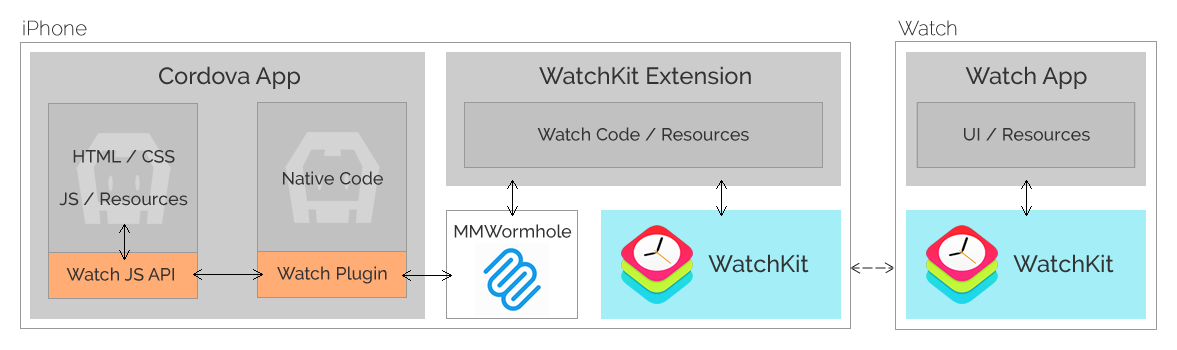
\includegraphics[width=0.9\textwidth]{data/bilder/apple-watch-plugin.png}
	\caption{Prinzip der Nachrichtenübermittlung mittels des Watch-Plugins \cite{CrossleyCordovaAppleWatchPlugin}}
	\label{fig:watchPlugin}
\end{figure}
%
MMWormhole erstellt dabei eine Brücke zwischen der App und ihrer Erweiterung mithilfe von \emph{App Groups}, die die iOS-Plattform seit Version 8 unterstützt. App Groups bieten mehreren Applikationen eines Entwicklers die Möglichkeit auf gemeinsame Daten zuzugreifen. So können auch Daten zwischen einer Extension und der eigentlichen iOS App ausgetauscht werden, was ansonsten aufgrund des Sandbox-Designs von iOS nicht möglich wäre. Das Watch Plugin steht also über die vom MMWormhole geschaffene Brücke mit dem gemeinsamen Speicherbereich von Apple Watch- und Ionic-App in einer Art Verbindung und kann so die bereits erwähnten Austauschmethoden anbieten.
%
% --------------------------------------------------------------------------------------------
%
\subsection{Grundsätzliche Methodik} 
%
Sowohl in der Ionic- als auch in der Watch-App muss innnerhalb von XCode die Nutzung einer gemeinsamen App Group mit fester Group Id definiert werden. Dies muss auch bei der Ionic-App manuell geschehen.
%
\subsubsection{Ionic-Seite}
%
Bevor eine Kommunikation zwischen den beiden Plattformen erfolgen kann muss eine Initialisierung stattfinden. Dazu wird eine Initialisierungsmethode \texttt{applewatch.init} aufgerufen:
\begin{lstlisting}[language=JavaScript]
applewatch.init(successHandler, errorHandler, appGroupId);
\end{lstlisting}
Dabei wird mittels des Parameters \texttt{appGroupId} die Application Group Id übergeben, die in XCode zuvor festgelegt wurde. Dies führt zur Bindung an die in XCode festgelegte Application Group.

Die Methode \texttt{sendMessage} ermöglicht es, nach erfolgreicher Initialisierung, Strings oder JSON-Objekte an die Watch App zu senden. JSON-Objekte werden dabei automatisch in Strings umgewandelt. 

\begin{lstlisting}[language=JavaScript]
applewatch.sendMessage(message, queueName, successHandler, errorHandler);
\end{lstlisting}
Der Parameter \texttt{queueName} muss dabei mit dem entsprechenden Listener der Watch App Funktion \texttt{MMWormhole.listenForMessageWithIdentifier} übereinstimmen. 

Mittels Listener-Funktionen auf Cordova-Seite können von der Apple Watch ausgesendete Nachrichten empfangen werden. Auch hier muss \texttt{queueName} mit der entsprechenden Methode auf Apple Watch Seite übereinstimmen.
\begin{lstlisting}[language=JavaScript]
applewatch.addListener(queueName, messageHandler);
applewatch.removeListener(queueName, successHandler, errorHandler);
\end{lstlisting}

Lokale Benachrichtigungen benötigen ebenfalls eine Registrierung und eine Erlaubnis für den Empfang lokaler Nachrichten. Dazu wird die Funktion \texttt{registerNotifications} erfragt:
\begin{lstlisting}[language=JavaScript]
applewatch.registerNotifications(successHandler, errorHandler);
\end{lstlisting}
Wird die Erlaubnis durch den Nutzer erteilt, so wird der \texttt{successHandler} mit true aufgerufen. Sonst wird der \texttt{errorHandler} mit false aufgerufen.

Mithilfe der Funktion \texttt{sendNotification} kann nun eine in einem JSON-Objekt (\texttt{payload}) gekapselte Nachricht an die Apple Watch gesendet werden.  
\begin{lstlisting}[language=JavaScript]
applewatch.sendNotification(successHandler, errorHandler, payload);
\end{lstlisting}

\emph{User defaults} werden dazu genutzt, um Nutzerdaten in Form von einzelnen Key-Value-Paaren zwischen der Watch-Extension und der iOS-App auszutauschen. Mithilfe der Funktion \texttt{sendUserDefaults} kann ein solches Key-Value-Paar gespeichert werden:
\begin{lstlisting}[language=JavaScript, breaklines=true]
applewatch.sendUserDefaults(successHandler, errorHandler, 
    { "myKey": "myValue" }, appGroupId);
\end{lstlisting}
Die Funktion \texttt{getUserDefaults} bietet Lesemöglichkeit:
\begin{lstlisting}[language=JavaScript]
applewatch.getUserDefaults(successHandler, errorHandler, 
    "myKey", appGroupId);
\end{lstlisting}
%
% --------------------------------------------------------------------------------------------
%
\subsubsection{Apple Watch-Seite}
Auf nativer Watchkit Extension Seite (hier beispielhaft in Swift) muss der Nachrichtenaustausch auch zunächst initialisiert werden:
\begin{lstlisting}[language=swift, breaklines=true]
let listeningSession = MMWormholeSession.sharedListeningSession();
listeningSession.activateSessionListening();

let wormhole = MMWormhole(applicationGroupIdentifier: "group.com.yourcompany", optionalDirectory: nil, transitingType: .SessionContext);
\end{lstlisting}

Die Methoden \texttt{passMessageObject} des MMWormhole-Objektes ermöglicht das Senden von Nachrichten. Mit Hilfe der Funktion \texttt{listenForMessageWithIdentifier} des MMWormholeSession-Objektes kann ein Listener erstellt werden:
\begin{lstlisting}[language=swift, breaklines=true]
wormhole.passMessageObject("titleString", identifier: "queueName");

listeningSession.listenForMessageWithIdentifier("queueName", listener: { (messageObject) -> Void in
    if let message: AnyObject = messageObject {
        // Do something
    }
});
\end{lstlisting}

Um auf die \emph{user defaults} auf Apple Watch-Seite zugreifen bietet das Framework die Klasse \texttt{NSUserDefaults}. Der bidirektionale Zugriff lässt sich wie folgt realisieren:
\begin{lstlisting}[language=swift, breaklines=true]
let userDefaults = NSUserDefaults(suiteName: "group.com.yourcompany")

var myValue: String? {
    userDefaults?.synchronize()
    return userDefaults?.stringForKey("myKey")
}
\end{lstlisting}
%
%\subsubsection{Beschränkung der austauschbaren Datengröße}
Problematisch ist, dass die Größe der Daten, die mithilfe dieses Plugins ausgetauscht werden können von den vom WatchKit-Framework gesetzten Grenzen für Nachrichten und UserDefaults stark limitiert ist. Eine einzelne Nachricht und jeder einzelne Eintrag in die UserDefaults hat eine maximale Größe von 65.5~KB. \cite{appleWatchPayloadMaximumDatatransfer}. Müssten größere Datenmengen ausgetauscht werden ginge dies nicht mit diesem Plugin. Stattdessen müsste ein Plugin entwickelt werden, was tatsächlichen Dateiaustausch ermöglicht, da für Dateiaustausch keine Beschränkung dieser Art existiert.
%
% --------------------------------------------------------------------------------------------
%
\subsection{Skizze einer möglichen Anwendung}
%
Um die hier beschriebene Funktionalität des Nachrichtenaustausches etwas besser zu verdeutlichen wird im folgenden die Nutzung des Plugins an einem Beispiel beschrieben werden.

Gegeben ist eine App, in der die Inhalte einer Tagung oder Messe dargestellt werden können. Diese App ist vollständig in Ionic geschrieben und liefert bereits einen Mechanismus, um die Daten der Veranstaltung mit einem Server abzugleichen und lokal zu speichern. Als Datenpersistierung wird eine Web SQL Datenbank verwendet. Diese wird gekapselt mit einem asynchronen objekt-relationalen JavaScript Mapper namens \emph{persistenceJS}, der auf dem Cordova SQLite Plugin aufbaut \cite{persistenceJSDoku}. In der Tagungsapp werden unter anderem Listen von Vorträgen und Diskussionsbeiträgen mit ihren Detailinformationen aufgelistet. Nutzer können dabei einzelne Beiträge als Favoriten markieren. Zudem können sich einzelne Teilnehmer mit anderen Teilnehmern und Ausstellern verabreden und Termine verabreden, die anschließend in einem App-eigenen Kalender dargestellt werden.

In einer möglichen zugehörigen Apple Watch Companion-App sollen ausgewählte Inhalte wie favorisierte Vorträge oder die Terminabsprachen auf der Watch-App aufgeführt werden. Die Apple Watch-App zeigt also einen sehr ausgewählten Teil der Daten der Ionic-App in angemessener Form. Ein Mockup für eine solche Realisierung ist in \fref{fig:AppleWatchMockup} dargestellt. 

\begin{figure}[htb] 
	\centering
	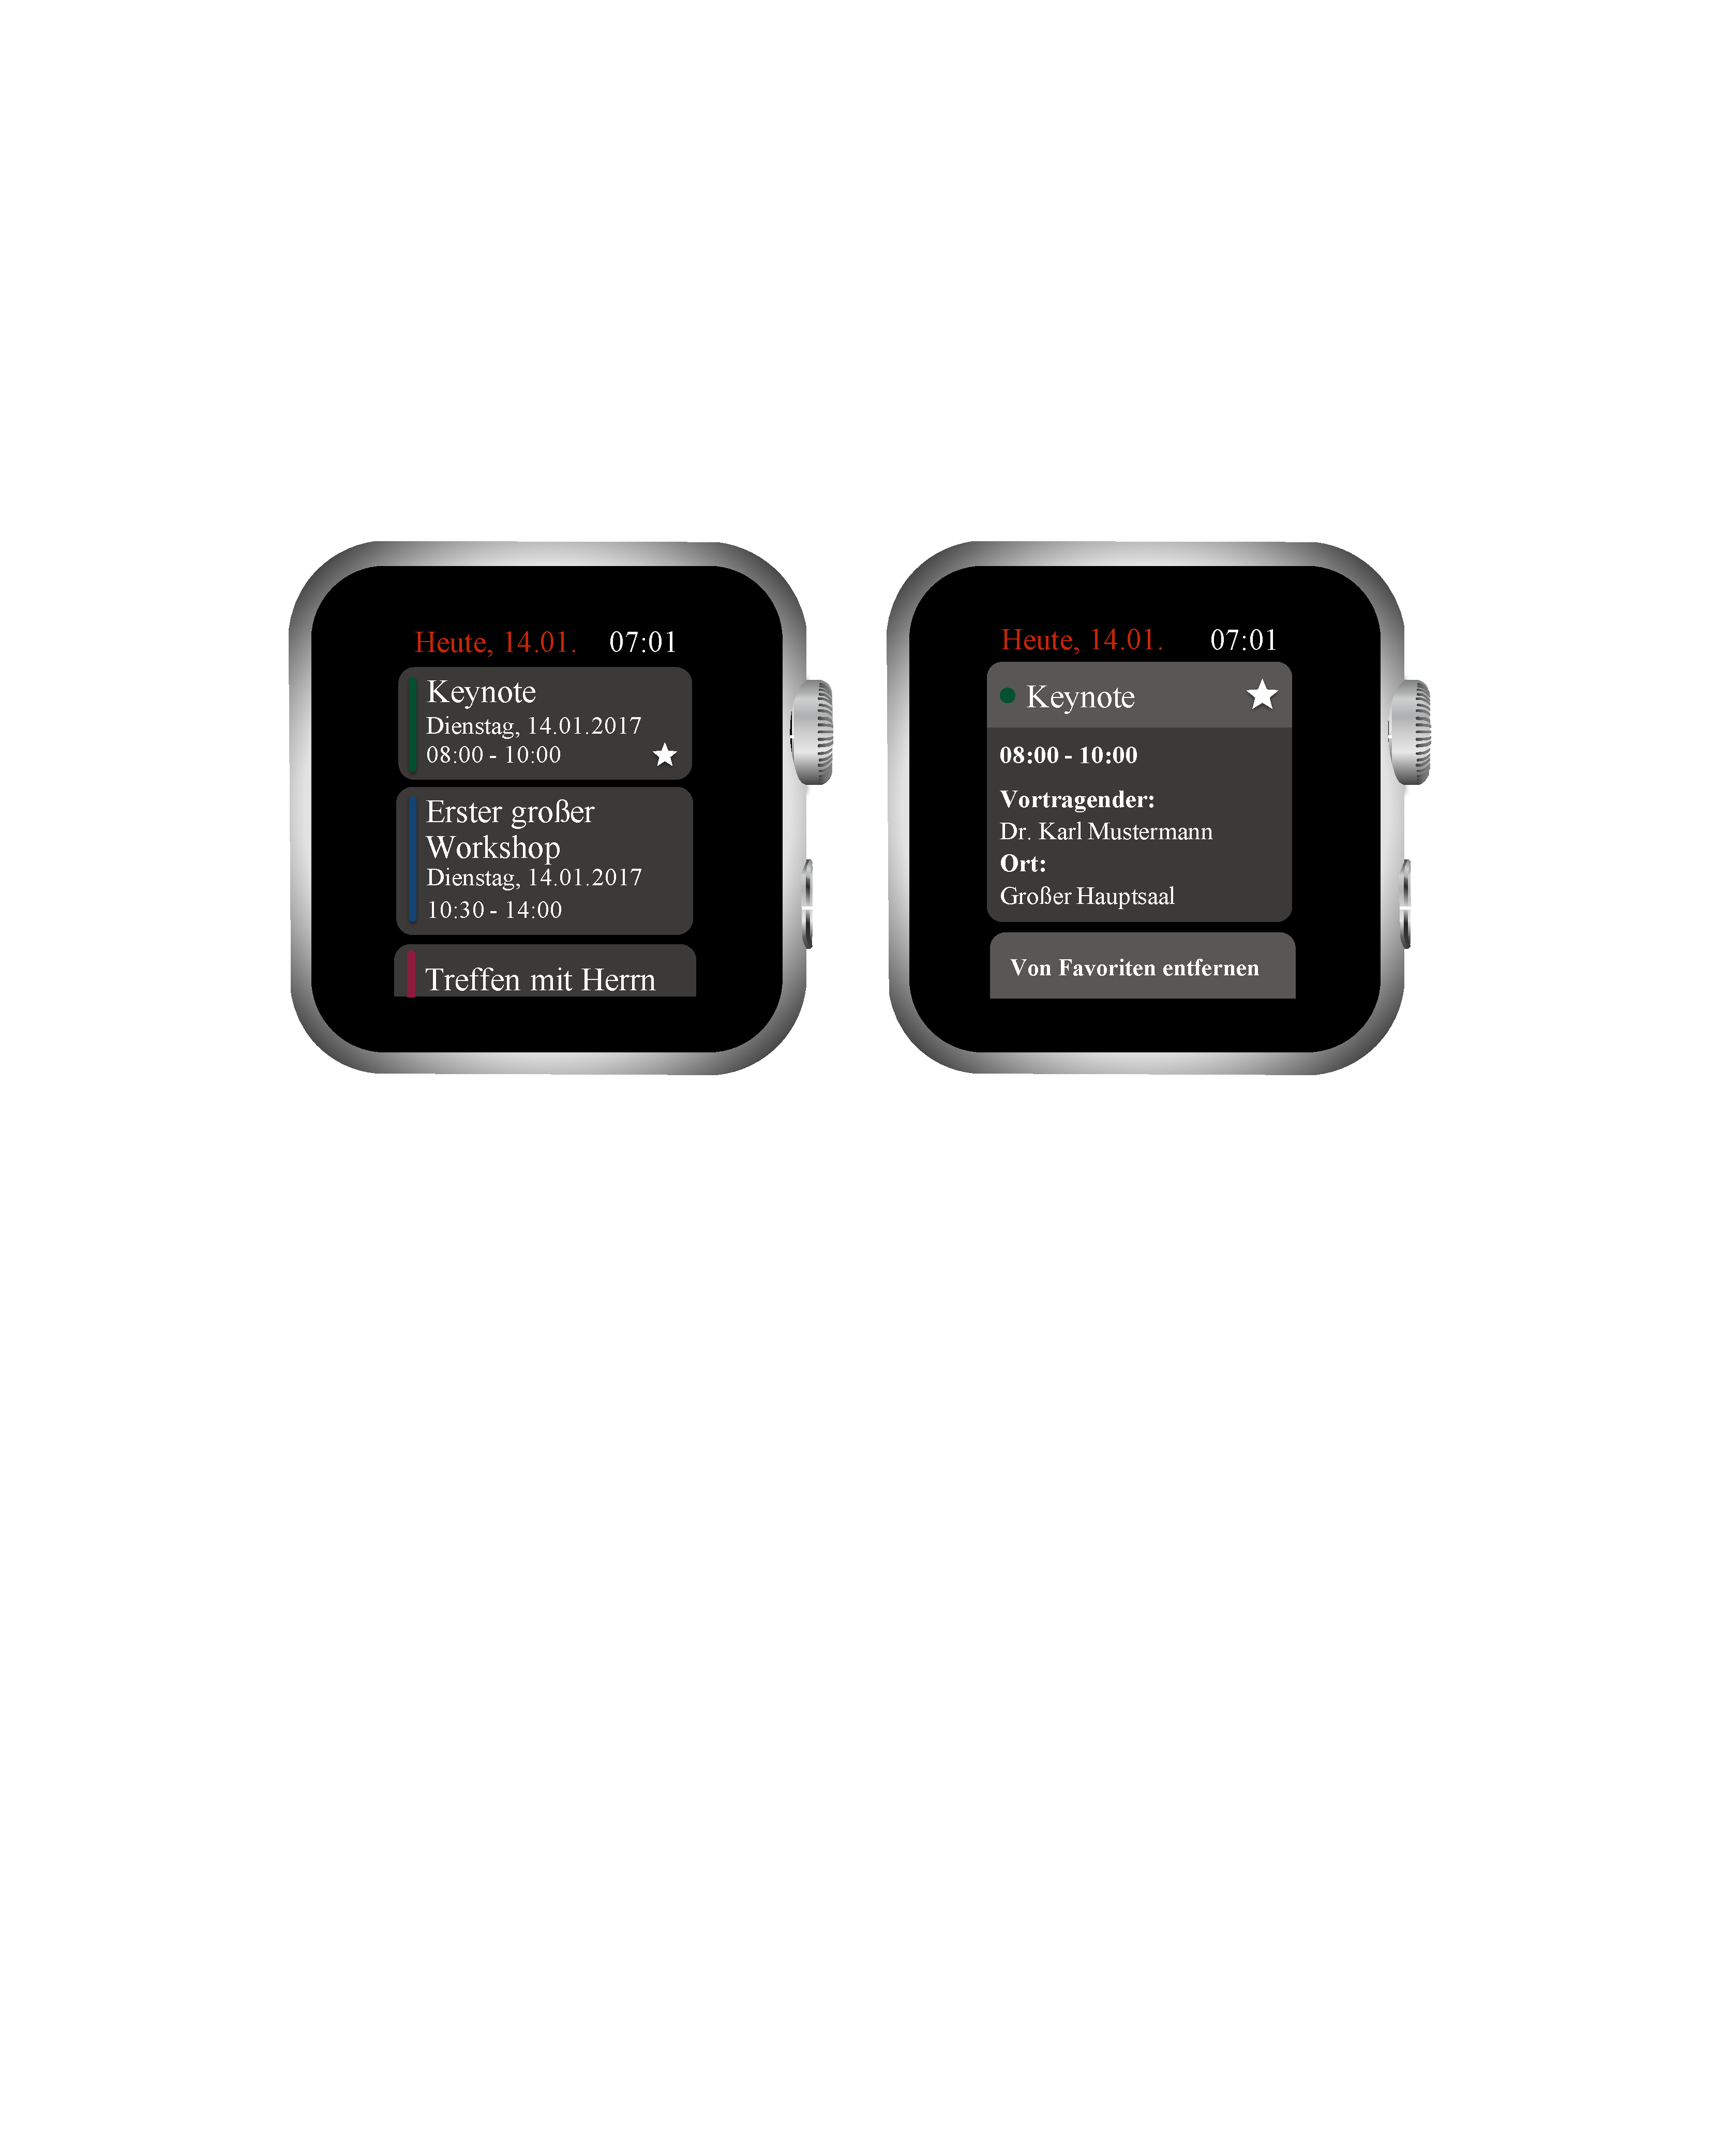
\includegraphics[width=0.6\textwidth]{data/bilder/AppleWatchMockup.pdf}
	\caption{Mockup einer möglichen Realisierung der Datenrepräsentation in einer Table View der Apple Watch und einer möglichen Detailansicht}
	\label{fig:AppleWatchMockup}
\end{figure}

Bei der Konzeption der Apple Watch-App ist darauf zu achten, dass die Smartwatch nur über einen sehr beschränkten Darstellungsbereich verfügt und somit Daten, die auf der Uhr dargestellt werden sollen, auf die wichtigsten Inhalte beschränkt werden müssen. Zudem ist die Eingabe nur über das kleine Display und die \enquote{Digital Crown} sowie den Knopf an der rechten Seite möglich. Apple hat dazu ein eigenes Dokument bereitgestellt, die watchOS Human Interface Guidelines \cite{appleWatchInterfaceGuidelines}, welche Konzeptprinzipien für gut bedienbare Watch-Apps zusammenfassen.

Die wichtigste Kernfunktionalität ist der Datenaustausch zwischen den beiden Plattformen.
Dieser lässt sich mithilfe des Plugins realisieren. Dazu muss der Datensatz aus der SQLite Datenbank der Ionic-App auf die Kerndaten, die in der Watch-App dargestellt werden sollen, reduziert werden. Anschließend müssen diese Datensätze in Form von JSON-Objekten umgesetzt werden und als String per Nachricht oder über die User defaults an die Apple Watch sendet. Dabei dürfen jedoch nur die nötigsten Daten an im JSON-Objekt gebündelt werden, da die Größe der übermittelten Daten beschränkt ist. Beispielhaft ist dieser Vorgang in Listing \ref{lst:watchCommunicationExample} dargestellt. Dem Codebeispiel liegt zugrunde, dass eine in XCode definierte appGroupId einzigartig ist und eine und über einen Mechanismus wie globale Variable oder einen entsprechenden Mechanismus global verfügbar gemacht wird. Genauso muss auf eine boolsche Variable successfullWatchInit global zugegriffen werden können. 

\begin{listing}[htb]
    \lstinputlisting{data/sourcecode/watchCodeExample.ts}
    \caption{Exemplarischer Datenaustausch für das Tagungsappbeispiel}
    \label{lst:watchCommunicationExample}
\end{listing}

Innerhalb der Apple Watch API gibt es die Klasse \texttt{NSJSONSerialization}, die genutzt werden kann um JSON-Objekte in \texttt{NSDictionary}-Objekte umzuwandeln und die nötigen Informationen für passende Objective~C- oder Swift-Objekte oder für die Speicherung in einer neuen Datenbankstruktur zu erhalten \cite{appleDokuJSONSerialization}. 

Diese Datensätze können anschließend in nativen Table Views der Apple Watch, wie im Mockup in \fref{fig:AppleWatchMockup} gezeigt, dargestellt werden.

